\documentclass[addpoints,12pt]{exam}
\usepackage{pgf-pie}
\usepackage{multicol}
\usepackage{arev}
\usepackage{graphicx,multicol}
\usepackage{charter,amsmath,amssymb}
\usepackage{eulervm}
\usepackage[letterpaper,margin=1in]{geometry}
\pagestyle{headandfoot}
\runningheadrule
\firstpageheader{\bf Math 104}{\bf Exam 1, Yellow Form}{\bf 4 February 2015}
\runningheader{\bf Math 104}
{\bf Exam One, Page \thepage\ of \numpages}
{\bf 4 February 2015}
\firstpagefooter{}{}{}
\runningfooter{}{}{}
\everymath{\displaystyle}
\begin{document}

\ifprintanswers\else
\begin{center}
\fbox{\fbox{\parbox{5.5in}{
This exam has \numquestions~questions.
It has been printed on \numpages~pages and is worth \numpoints~points.
Answer all the questions below in the spaces provided.
In order to receive maximum credit, you must
clearly indicate how you arrived at your answers.
By signing below, you pledge that
\begin{enumerate}
\item you will not communicate to any person in any conceivable way anything
about the contents of this exam
until all students have taken the exam, and
\item in taking this exam now,
you have not been the recipient of such communication from anyone else.
\end{enumerate}}}}
\end{center}
\vspace{.2in}
\makebox[\textwidth]{Your signature:\enspace\hrulefill}\\
\vspace{.2in}\\
\makebox[\textwidth]{Your name:\enspace\hrulefill}\\
\vspace{.2in}\\
\makebox[\textwidth]{Your student ID number:\enspace\hrulefill}
\fi

\begin{questions}

\question[15] A die is rolled and the number
showing on the top face observed. Determine the probability
of each of the following events.
\begin{parts}
\part The number is $1$
\begin{solution}[1.25in]$\frac{1}{6}$\end{solution}
\part The number is greater than $1$
\begin{solution}[1.25in]$\frac{5}{6}$\end{solution}
\part The number is even
\begin{solution}[1.25in]$\frac{3}{6}=\frac{1}{2}$\end{solution}
\end{parts}
\ifprintanswers\else\newpage\fi

\question[10] The results of the first quiz in Math~104 are
shown in the table below. For each possible score, the number
of students receiving that score is shown directly below
the score.
\[\begin{array}{c|cccccccccc}
\text{Score}&2&3&4&5&6&7&8&9&10\\\hline
\text{Frequency}&4&5&9&21&25&20&21&19&16\\
\end{array}\]
Calculate the empirical probability that a randomly
selected Math~104 student scored eight or higher
on the first quiz.
\begin{solution}[2in]
\[\frac{21+19+16}{4+5+9+21+25+20+21+19+16}
=\frac{56}{140}=\frac{2}{5}=0.4\]
\end{solution}

\question[15] Suppose that a woman has genotype $\mathbold{cC}$
and her husband has genotype $\mathbold{CC}$ for a
genetically inherited disorder.
If they decide to become parents, calculate the
probability that their child will
have the following genotypes.
\begin{parts}
\part $\mathbold{cc}$
\begin{solution}[1.25in]
The Punnett square is
$\begin{array}{c|cc}
&\mathbold{c}&\mathbold{C}\\\hline
\mathbold{C}&\mathbold{Cc}&\mathbold{CC}\\
\mathbold{C}&\mathbold{Cc}&\mathbold{CC}\end{array}$
so $\mathbold{cc}$ occurs with probability~0.
\end{solution}
\part either $\mathbold{Cc}$ or $\mathbold{cC}$
\begin{solution}[1.25in]$\frac{1}{2}$\end{solution}
\part $\mathbold{CC}$
\begin{solution}[1.25in]$\frac{1}{2}$\end{solution}
\end{parts}
\ifprintanswers\else\newpage\fi

\question[25]
Marcus and Alex are playing the following game repeatedly.
Marcus selects a card at random from a deck of cards.
If the card is a picture card, then Alex pays Marcus $\$6$.
Otherwise Marcus pays Alex $\$3$.
A {\em picture card} is either a Jack, Queen, or King.
Then the card is reinserted into the deck and the
game repeated.
\begin{parts}
\part Calculate the probability of drawing a picture card.
\begin{solution}[.75in]$\frac{3}{13}$\end{solution}
\part Calculate the {\bf odds against} drawing a picture card.
\begin{solution}[.75in]
$\frac{10/13}{3/13}=\frac{10}{3}$ so the odds
against drawing a picture card are $10:3$.
\end{solution}
\part Calculate the expected proceeds for Marcus.
\begin{solution}[.75in]
$6\left(\frac{3}{13}\right)-3\left(\frac{10}{13}\right)
=-\frac{12}{13}\approx -0.93$
\end{solution}
\part How can the payments be changed so that the game
will be fair to both players?
\begin{solution}[1in] Change Alex's payment to $\$10$. Then
Marcus's expectation is
\[10\left(\frac{3}{13}\right)-3\left(\frac{10}{13}\right)=0.\]
\end{solution}
\end{parts}

\question[20] To raise money the volleyball team sells
800~raffle tickets
for $\$3$ each. They will randomly select
a ticket holder to receive a prize of $\$200$.
\begin{parts}
\part Calculate the expected proceeds for someone
who buys a ticket.
\begin{solution}[.75in]
$197\left(\frac{1}{800}\right)-3\left(\frac{799}{800}\right)
=-\frac{2200}{800}=-\frac{11}{4}=-2.75$
\end{solution}
\part Calculate the expected proceeds for the volleyball team.
\begin{solution}[.75in]
$800\cdot 3-200=2200$
\end{solution}
\part Calculate the fair ticket price.
\begin{solution}[.75in]
$3-\frac{11}{4}=\frac{1}{4}=0.25$
\end{solution}
\end{parts}
\ifprintanswers\else\newpage\fi

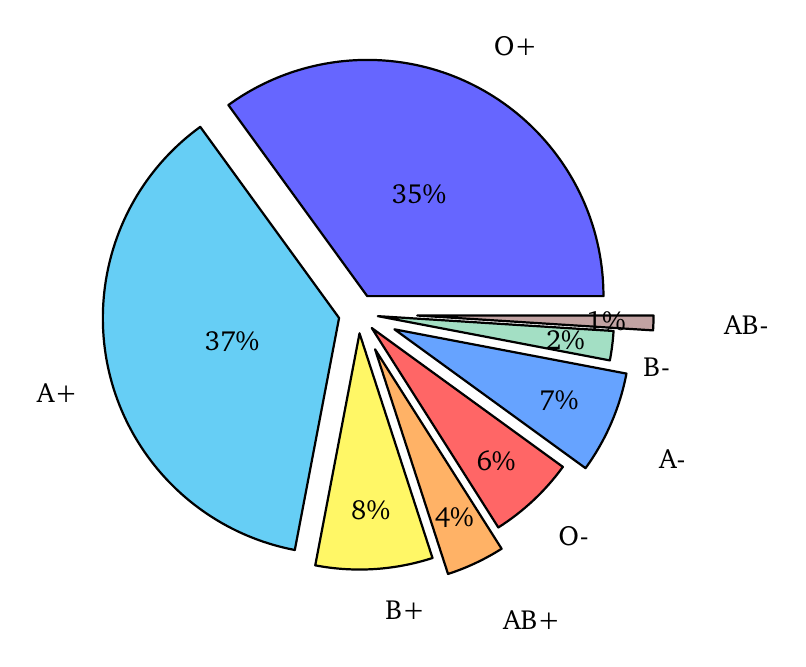
\begin{tikzpicture}
\pie[explode={.25,.25,.25,.5,.25,.5,.25,.75}]
{35/O+,37/A+,8/B+,4/AB+,6/O-,7/A-,2/B-,1/AB-}
\end{tikzpicture}

\question[15]
The chart above shows the distribution
of blood types of residents of Denmark.
\begin{parts}
\part If a Danish individual is selected at random,
what is the probability that he or she
does {\bf not} have blood type {A+}?
\begin{solution}[.75in]$1-0.37=0.63$\end{solution}
\part What are the {\bf odds against} a randomly
selected Danish individual having blood type {O+}?
\begin{solution}[.75in]
$\frac{0.65}{0.35}=\frac{13}{7}$ so the odds against
{O+} are $13:7$.
\end{solution}
\part What is the probability that a randomly
selected Danish individual has blood type either
{O+} or {O-}?
\begin{solution}[.75in]$0.35+0.06=0.41$\end{solution}
\end{parts}
\end{questions}

\vfill
\ifprintanswers\else
\begin{center}{\bf End of exam.
Do not write anything in the table below.}\\
\gradetable[h][questions]\end{center}
\fi

\end{document}
